\section{Results}
\label{sec:results}

\subsection{Architecture and Structured-State Controls}

The most important result is the B/G/C architecture matrix. Adding typed PAT-ER
registers to the same pretrained backbone improves primitive macro-F1 by 0.209
and role-to-primitive macro-F1 by 0.091 over the token-state baseline across
eight seeds. A generic-register control also improves some metrics over token
pooling, so it is not a strawman. However, typed PAT-ER adds a further
significant increment over generic registers: +0.116 primitive macro-F1,
+0.110 role-to-primitive macro-F1, +0.273 primitive-contradiction recall, and
+0.227 primitive-contradiction F1 on shallow OWA validation data. The same
ordering holds on deep/CWA validation.

\begin{figure}[H]
\centering
\resizebox{0.95\textwidth}{!}{%
\begin{tikzpicture}[font=\small, >=Latex]
  \draw[->] (0,0) -- (10.8,0) node[right]{metric};
  \draw[->] (0,0) -- (0,5.2) node[above]{score};
  \foreach \y/\lab in {0/0.0,1/0.2,2/0.4,3/0.6,4/0.8,5/1.0}
    {\draw (-0.08,\y) -- (0.08,\y) node[left=4pt]{\lab};}

  % scale: score * 5
  \foreach \x/\name/\b/\g/\c in {
    1.0/Primitive F1/3.41/3.88/4.46,
    4.0/r2p F1/4.08/3.98/4.53,
    7.0/Contra F1/1.60/2.58/3.71
  }{
    \draw[fill=gray!35] (\x,0) rectangle ++(0.42,\b);
    \draw[fill=orange!55] (\x+0.5,0) rectangle ++(0.42,\g);
    \draw[fill=blue!55] (\x+1.0,0) rectangle ++(0.42,\c);
    \node[rotate=20, anchor=east] at (\x+1.45,-0.25) {\name};
  }
  \node[fill=gray!35, draw, minimum width=5mm] at (8.9,4.75) {};
  \node[right] at (9.25,4.75) {B: Qwen + labels};
  \node[fill=orange!55, draw, minimum width=5mm] at (8.9,4.35) {};
  \node[right] at (9.25,4.35) {G: generic registers};
  \node[fill=blue!55, draw, minimum width=5mm] at (8.9,3.95) {};
  \node[right] at (9.25,3.95) {C: typed PAT-ER};
\end{tikzpicture}%
}
\caption{Contribution matrix graph. Generic learned registers improve some metrics over token pooling, but typed PAT-ER registers add a further gain, especially on the role-to-primitive and contradiction axes.}
\label{fig:contribution_matrix}
\end{figure}

\begin{table}[H]
\caption{Primary architecture result on shallow OWA validation data, eight seeds. CIs are paired bootstrap 95\% intervals for B to C deltas.\label{tab:architecture_matrix}}
\footnotesize
\begin{tabularx}{\textwidth}{@{}p{0.28\linewidth}p{0.18\linewidth}p{0.18\linewidth}p{0.15\linewidth}X@{}}
\toprule
\textbf{Metric} & \textbf{B: Qwen + labels} & \textbf{C: PAT-ER registers} & \textbf{Delta} & \textbf{95\% CI} \\
\midrule
Primitive macro-F1 & 0.682 $\pm$ 0.027 & \textbf{0.891 $\pm$ 0.022} & \textbf{+0.209} & [0.182, 0.237] \\
Role-to-primitive macro-F1 & 0.815 $\pm$ 0.005 & \textbf{0.905 $\pm$ 0.029} & \textbf{+0.090} & [0.074, 0.110] \\
Contradiction recall & 0.242 $\pm$ 0.110 & \textbf{0.735 $\pm$ 0.202} & +0.492 & [0.280, 0.705] \\
Entailment refuted recall & 0.021 $\pm$ 0.059 & \textbf{0.427 $\pm$ 0.433} & +0.406 & [0.167, 0.677] \\
LM loss & 2.563 $\pm$ 0.059 & 2.555 $\pm$ 0.057 & $\approx$0 & not material \\
\bottomrule
\end{tabularx}
\end{table}


\begin{table}[H]
\caption{Paired seed deltas for the structured-state control. Bold entries have bootstrap 95\% confidence intervals excluding zero. The G $\rightarrow$ C rows test whether typed PAT-ER flow improves over generic learned registers.\label{tab:reviewer_deltas}}
\scriptsize
\resizebox{\textwidth}{!}{%
\begin{tabular}{@{}llllll@{}}
\toprule
\textbf{Delta} & \textbf{Primitive macro-F1} & \textbf{R2P macro-F1} & \textbf{Contradiction recall} & \textbf{Contradiction F1} & \textbf{Entailment-refuted recall} \\
\midrule
B $\rightarrow$ G, shallow & \textbf{+0.094 [0.060, 0.130]} & $-0.020$ [$-0.062$, 0.020] & \textbf{+0.188 [0.023, 0.364]} & \textbf{+0.195 [0.072, 0.316]} & +0.073 [$-0.062$, 0.281] \\
G $\rightarrow$ C, shallow & \textbf{+0.116 [0.080, 0.151]} & \textbf{+0.110 [0.064, 0.160]} & \textbf{+0.273 [0.148, 0.398]} & \textbf{+0.227 [0.099, 0.380]} & +0.333 [$-0.031$, 0.688] \\
B $\rightarrow$ C, shallow & \textbf{+0.209 [0.182, 0.237]} & \textbf{+0.091 [0.074, 0.110]} & \textbf{+0.460 [0.278, 0.636]} & \textbf{+0.422 [0.277, 0.561]} & \textbf{+0.406 [0.167, 0.677]} \\
G $\rightarrow$ C, deep/CWA & \textbf{+0.097 [0.070, 0.125]} & \textbf{+0.091 [0.048, 0.136]} & \textbf{+0.307 [0.182, 0.420]} & \textbf{+0.245 [0.146, 0.354]} & \textbf{+0.398 [0.057, 0.761]} \\
\bottomrule
\end{tabular}%
}
\end{table}


The role-to-primitive contradiction axis is the clearest discriminator between
generic and typed structure. Generic registers are worse than token pooling on
role-to-primitive contradiction F1, while typed PAT-ER recovers it. In paired
seed deltas, B $\rightarrow$ G is negative on this axis ($-0.273$, 95\% CI
[$-0.443$, $-0.097$]), whereas G $\rightarrow$ C is strongly positive
(+0.483, 95\% CI [0.239, 0.733]). This indicates that undifferentiated register
capacity cannot substitute for typed event-role $\rightarrow$ primitive
coupling.

\subsection{Warm-Started Usable Model}

Condition C proves the architecture. Condition D is the usable model: it
retains much of the side-state behavior while reducing LM loss from 2.555 to
1.344. The warm-start sequence was not a single lucky tuning run. It required
four validated stages: frozen-backbone register learning, safe register-only
injection, upper-layer adapter opening, and KL-guarded top-layer adaptation.

\begin{figure}[H]
\centering
\resizebox{\textwidth}{!}{%
\begin{tikzpicture}[
  font=\small,
  >=Latex,
  stagebox/.style={draw, rounded corners=2pt, minimum width=34mm, minimum height=12mm, align=center, fill=blue!8},
  pass/.style={draw, rounded corners=2pt, minimum width=34mm, minimum height=12mm, align=center, fill=green!14},
  arr/.style={->, line width=0.8pt}
]
\node[stagebox] (s3) {Stage 3\\frozen backbone\\registers learn};
\node[stagebox, right=8mm of s3] (s4) {Stage 4\\register-only\\safe injection};
\node[stagebox, right=8mm of s4] (s5a) {Stage 5A\\upper adapters\\selective open};
\node[pass, right=8mm of s5a] (s5b) {Stage 5B\\top-2 backbone\\KL guarded};
\draw[arr] (s3) -- (s4);
\draw[arr] (s4) -- (s5a);
\draw[arr] (s5a) -- (s5b);
\node[below=7mm of s3] {primitive 0.006 $\to$ 0.884};
\node[below=7mm of s4] {LM delta within guard};
\node[below=7mm of s5a] {layers 21--27 adapt};
\node[below=7mm of s5b] {LM loss 1.344};
\end{tikzpicture}%
}
\caption{Warm-start validation sequence. The usable model is obtained only after safe injection, selective adapter opening, and KL-guarded top-layer adaptation.}
\label{fig:warmstart_stages}
\end{figure}

\begin{table}[H]
\caption{Warm-start validation stages.\label{tab:warmstart_stages}}
\footnotesize
\begin{tabularx}{\textwidth}{@{}p{0.16\linewidth}p{0.39\linewidth}X@{}}
\toprule
\textbf{Stage} & \textbf{What was tested} & \textbf{Key result} \\
\midrule
Stage 3 & Train PAT-ER registers on frozen Qwen3 backbone & Primitive macro-F1 0.006 to 0.884; LM unchanged \\
Stage 4 & Open safe register-only injection & LM delta within guard; KL below threshold; generation modulated \\
Stage 5A & Open upper-layer PAT-ER adapters & Layers 21--27 adapt; lower layers remain unchanged \\
Stage 5B & Unfreeze top two Qwen layers under KL guard & Backbone adapts safely; KL guard never triggers \\
\bottomrule
\end{tabularx}
\end{table}



\subsection{Decoupled Product Interface}

The first shared-layer interface SFT improved tool calls but damaged the
role-to-primitive bridge by 0.094. The accepted solution decouples product
generation from side-state measurement: train copied top decoder blocks only in
\texttt{interface\_mode}; keep base mode byte-identical to Condition D.

\begin{figure}[H]
\centering
\resizebox{0.9\textwidth}{!}{%
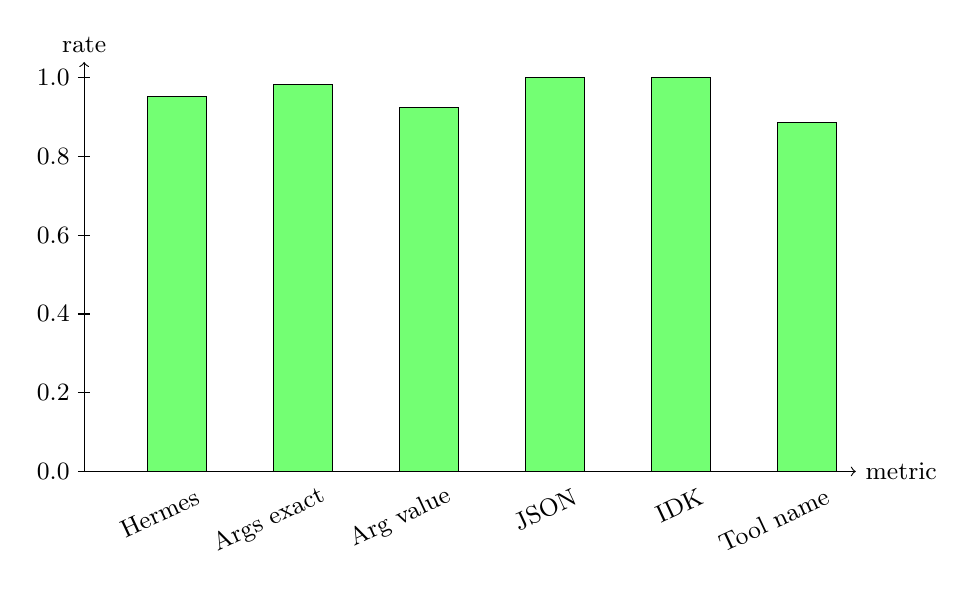
\begin{tikzpicture}[font=\small]
  \draw[->] (0,0) -- (9.8,0) node[right]{metric};
  \draw[->] (0,0) -- (0,5.2) node[above]{rate};
  \foreach \y/\lab in {0/0.0,1/0.2,2/0.4,3/0.6,4/0.8,5/1.0}
    {\draw (-0.08,\y) -- (0.08,\y) node[left=4pt]{\lab};}
  \foreach \x/\name/\val in {
    0.8/Hermes/4.76,
    2.4/Args exact/4.91,
    4.0/Arg value/4.62,
    5.6/JSON/5.00,
    7.2/IDK/5.00,
    8.8/Tool name/4.43
  }{
    \draw[fill=green!55] (\x,0) rectangle ++(0.75,\val);
    \node[rotate=25, anchor=east] at (\x+0.75,-0.25) {\name};
  }
\end{tikzpicture}%
}
\caption{Decoupled interface metrics on 242 held-out prompts. Tool-name exact copying is the remaining boundary; schema-grounded calls, exact arguments, JSON, and IDK pass.}
\label{fig:interface_metrics}
\end{figure}


\begin{table}[H]
\caption{Decoupled interface evaluation on 242 held-out prompts, three seeds.\label{tab:interface_eval}}
\footnotesize
\begin{tabularx}{\textwidth}{@{}p{0.34\linewidth}p{0.18\linewidth}p{0.16\linewidth}X@{}}
\toprule
\textbf{Metric} & \textbf{Result} & \textbf{Target} & \textbf{Verdict} \\
\midrule
Hermes parse & \textbf{0.952} & $\ge$0.90 & Pass \\
Tool arguments exact & \textbf{0.981} & $\ge$0.80 & Pass \\
Argument value accuracy & 0.923 & -- & Reported \\
JSON valid / required keys & \textbf{1.000 / 1.000} & $\ge$0.95 & Pass \\
IDK precision/recall/F1 & \textbf{1.000} & 1.000 & Pass \\
Base-mode primitive/r2p/LM vs D & byte-identical & exact & Pass \\
Tool-name exact accuracy & 0.886 & $\ge$0.90 & Boundary \\
\bottomrule
\end{tabularx}
\end{table}



On 242 held-out prompts across three seeds, the decoupled interface reaches
Hermes parse 0.952, exact argument correctness 0.981, JSON validity 1.000, and
IDK F1 1.000. Exact unseen tool-name copying remains imperfect at 0.886. This is
reported as an interface limit, not as a side-state regression, because base
mode is identical to Condition D.

\subsection{Negative Results}

The negative result record is central to the claim because it shows that the
reported path is not merely the last surviving configuration. Several plausible
alternatives failed for diagnosed reasons.

\begin{figure}[H]
\centering
\resizebox{\textwidth}{!}{%
\begin{tikzpicture}[
  font=\small,
  bad/.style={draw, rounded corners=2pt, minimum width=32mm, minimum height=10mm, align=center, fill=red!10},
  good/.style={draw, rounded corners=2pt, minimum width=32mm, minimum height=10mm, align=center, fill=green!12},
  arr/.style={->, line width=0.8pt}
]
\node[bad] (a) {External-style\\synthetic aug\\rejected};
\node[bad, right=6mm of a] (b) {SNLI explicit\\conflict\\rejected};
\node[bad, right=6mm of b] (c) {Fact pointers\\item heads\\rejected};
\node[bad, below=8mm of b] (d) {Shared-layer\\interface SFT\\bridge cost};
\node[good, right=10mm of d] (e) {Decoupled\\interface mode\\accepted};
\draw[arr] (a) -- (b);
\draw[arr] (b) -- (c);
\draw[arr] (d) -- (e);
\node[draw, dashed, rounded corners=2pt, fit=(a)(b)(c)(d)(e), inner sep=4mm,
      label={[font=\small]above:Audit-disciplined gate record}] {};
\end{tikzpicture}%
}
\caption{Negative-result map. Plausible additions were tested and rejected when they harmed the targeted slice or damaged the bridge.}
\label{fig:negative_results}
\end{figure}


\begin{table}[H]
\caption{Documented negative results and retained decision.\label{tab:negative_results}}
\footnotesize
\begin{tabularx}{\textwidth}{@{}p{0.25\linewidth}p{0.38\linewidth}X@{}}
\toprule
\textbf{Gate} & \textbf{Observed failure} & \textbf{Decision} \\
\midrule
Synthetic external-style augmentation & Hurt the real external slice even when synthetic-ext spans were learnable & Do not merge; use only for eval/curriculum \\
SNLI / explicit-conflict NLI & Improved its own conflict form but damaged ProofWriter contradiction & Reject from main mix \\
Token fact pointers & Failed to learn distributed fact sets and regressed MP & Gate off \\
Evidence-item heads & Supporting item learned weakly; contradicting item did not learn & Gate off \\
Deep/CWA from-scratch data & Improved in-distribution deep/CWA but destroyed shallow contradiction & Do not merge for 450M-from-scratch \\
Stage 6B aux-refresh & Catastrophic forgetting of contingency and axiom boundaries & Reject E \\
Shared-layer interface SFT & Tool calls improved but role-to-primitive regressed by 0.094 & Replace with decoupled interface mode \\
\bottomrule
\end{tabularx}
\end{table}



The pattern is consistent. Synthetic substitutes for real external data hurt
the real external slice. Explicit-conflict NLI helps its own surface
contradiction but hurts ProofWriter contradiction. Fact-level pointer heads do
not help at the available refutation density. Aux-refresh on the adapted
backbone causes class forgetting. Shared-layer SFT improves output formatting
but damages the bridge. The accepted recipe avoids these failure modes by
keeping architecture measurement and product generation decoupled.
